\section{How to Invigilate Exams}

\subsection{How to Participate}
If a fully funded PhD student has not completed the required TA hours, the school will assign you to invigilate exams. There are only two invigilation sessions per semester: midterm and final exams. Due to the pandemic in recent years, there haven't been in-person exams for a while.

When there are many exams and not enough staff or fully funded PhD students, non-fully-funded PhD students can also sign up to be invigilators. The specific method is to wait for the school's email invitation, which will include a link for you to choose your preferred time. After selection, you can check your specific invigilation schedule on e-bridge in a few days.

The invigilation wage rate in 2022 is 60 RMB per hour. The preparatory work is minimal, and during invigilation, you basically just walk around. It's relatively easy and a good way for non-fully-funded students to earn money.

\subsection{Specific Steps}
First, the school provides invigilation training, which can be found under "Assessment and invigilation" in the email titled \textit{Teaching Assistant (TA) Training Programme}, or you can check your LMO. If you've never attended before, you might consider attending to get a general idea of the process.

An exam hall's invigilation is divided into senior invigilator (staff) and invigilation assistant (PhD students).

I've summarized the invigilation process as follows:
\begin{enumerate}
    \item The invigilation training mentioned above, although you don't have to attend every time, it's customary to receive the [invigilator ID badge] during each semester's training. You must wear it during invigilation and return it afterward. So even if you don't want to attend, you at least need to go once to get your badge. If you're lazy (like me), you can usually have other colleagues who are also invigilating pick it up for you (usually one person from the office collects all badges).
    \item Check your invigilation schedule on e-bridge, as shown below:
        \begin{figure}[H]
            \centering
            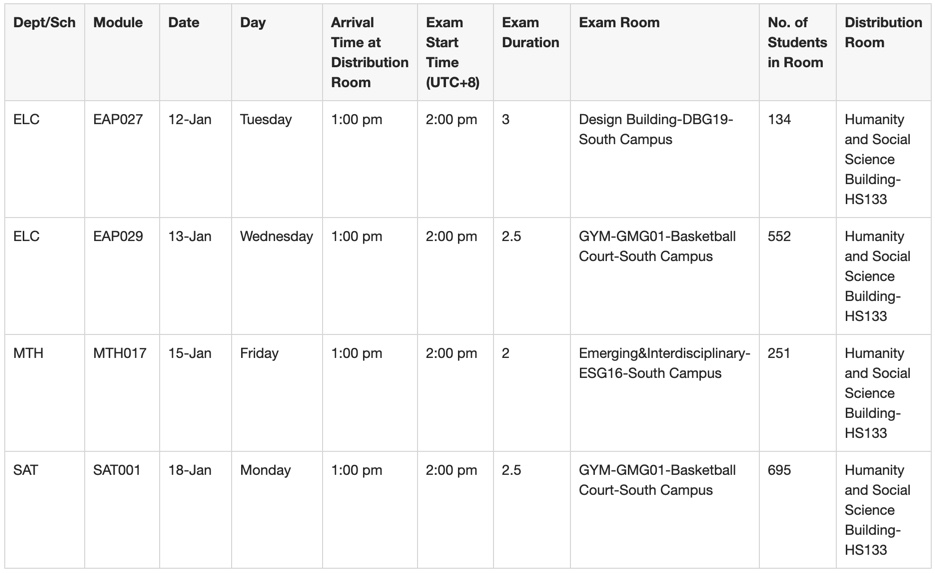
\includegraphics[width=0.5\columnwidth]{author-folder/Kai.Wu/invigi-table.jpg}
        \end{figure}
    \item First part of invigilation: pre-exam preparation. Before the exam starts, pay attention to the two columns in the table above: "Arrive Time at Distribution Room" and "Distribution Room". At the specified time, go to sign in and collect exam papers in advance. You will then get MCQ cards, answer booklets, exam attendance lists, small white cards, clay, and other materials to take to the exam hall.
    \item Upon arriving at the exam hall, the first task is to post materials. In the list of examinees, there is a version sorted by student number to be posted on the door for students to find their seats (other versions sorted by seat number are for invigilators). Separate each page of this list and use clay to stick them on the exam hall door or wall.
    \item Then start distributing answer booklets and answer sheets according to the seating plan.
    \item Generally, there will be multiple invigilators in an exam hall. When other invigilators arrive, assign some of the tasks of distributing answer booklets and sheets to them. Then, discuss with them to assign each person a specific area to be responsible for, including invigilation patrols and collecting materials.
    \item The senior invigilator (the staff) will bring the exam papers, and you can help the teacher distribute them. If the senior invigilator hasn't arrived 20 minutes before the exam starts, you need to contact the staff in the invigilator WeChat group to remind them.
    \item All materials (exam papers, answer sheets, MCQs, etc.) must be distributed 15 minutes before the start. Allow students to enter the exam hall 15 minutes before the exam.
    \item When multiple invigilators are present, generally leave at least one invigilator at each entrance to check student IDs. Students without student IDs or ID cards are not allowed to enter. Other invigilators can walk around inside the exam hall, paying special attention to ensuring students do not open the exam papers before the exam starts. If discovered, you need to stop it immediately. If there are many students doing this, ask the senior invigilator to warn them. To prevent loss, students' backpacks should not be placed outside the exam hall; they should be placed at the front or back of the hall.
    \item After the senior invigilator announces the start of the exam, for your responsible area, record any late-arriving students. You can note this on your invigilator attendance list.
    \item After the exam starts, walk around freely and exercise your authority as an invigilator. Focus on checking students' belongings to see if they have cheat sheets on their hands or paper slips. During invigilation, you are not allowed to use your phone or chat; you need to observe whether students are cheating. If cheating is encountered, you need to point it out on the spot, stop the student's exam, and make a note on their exam paper.
    \item 30 minutes after the exam starts, collect the small white cards (a card specifically for writing names, student numbers, etc.). After collecting, record the absent students in your area.
    \item If students need to borrow pens, pencils, or erasers, ask the senior invigilator how to handle it. If a student needs to go to the restroom, an invigilator needs to accompany them (just to the restroom entrance is sufficient), and accompany them back. In principle, only one student can go to the restroom at the same time. If a second student needs to go, they must wait until the first student returns.
    \item Finally, when the exam ends, collect all materials, including scratch paper (if any). Students must wait until you have finished collecting and counted everything accurately before they can leave.
    \item After the exam, tally the number of attendees, late arrivals, and absentees, and have the senior invigilator record it on the record sheet. Finally, there are two sheets that require the signatures of all invigilators. Only with these two signatures plus the initial sign-in will your work be successfully recorded.
    \item Then it's time to say goodbye. The senior invigilator will take away the answer booklets and MCQs. You need to return the two signed sheets and all materials the senior invigilator didn't take (including exam papers, scratch paper, etc.) to the place where you initially signed in. If this is your last invigilation of the semester, you need to return your invigilator ID badge.
\end{enumerate}

\emptyline{}
Finally, I'd like to share a checklist I use after invigilating more than a dozen times:

\begin{enumerate}
    \item When picking up materials, check the number of invigilators to facilitate dividing areas.
    \item Post the seating charts at the exam hall.
    \item Confirm with the senior invigilator:
    \begin{enumerate}
        \item Should the answer booklets be collected in order? If yes, at the end of the exam, do not let students pass the papers; absent students and those who submit early should also leave their papers on the desk.
        \item Stickers? If needed, have students attach them at the end of the exam.
        \item Whether to record restroom visits and start/end times.
        \item How to handle absentees (fill in information on the small white card and answer booklet, write "Absent" on the answer booklet).
    \end{enumerate}
    \item After receiving seat numbers, divide areas according to the number of invigilators. The roles in each area include everything except collecting papers:
    \begin{enumerate}
        \item Before the exam: Distribute papers, check if students are seated correctly, ensure students do not open the white question booklets.
        \item Letting students in: Check student IDs at the entrance.
        \item First 30 minutes: Check seating, record late arrivals.
        \item At 30 minutes: Record absentees, collect small white cards, then fill in the student attendance sheet.
        \item Restroom visits: Record seat number, start and end times.
        \item 15 minutes before end: Record seat numbers and count of students who submit early.
    \end{enumerate}
    \item Before finishing: Remind the teacher to have students attach the answer booklet.
    \item After finishing: Collect answer sheets in order, count your own portion, then combine and randomly count a portion.
    \item Summary list: Number of students, absentees, early submissions, remaining, special cases.
\end{enumerate}

\begin{figure}[H]
    \centering
    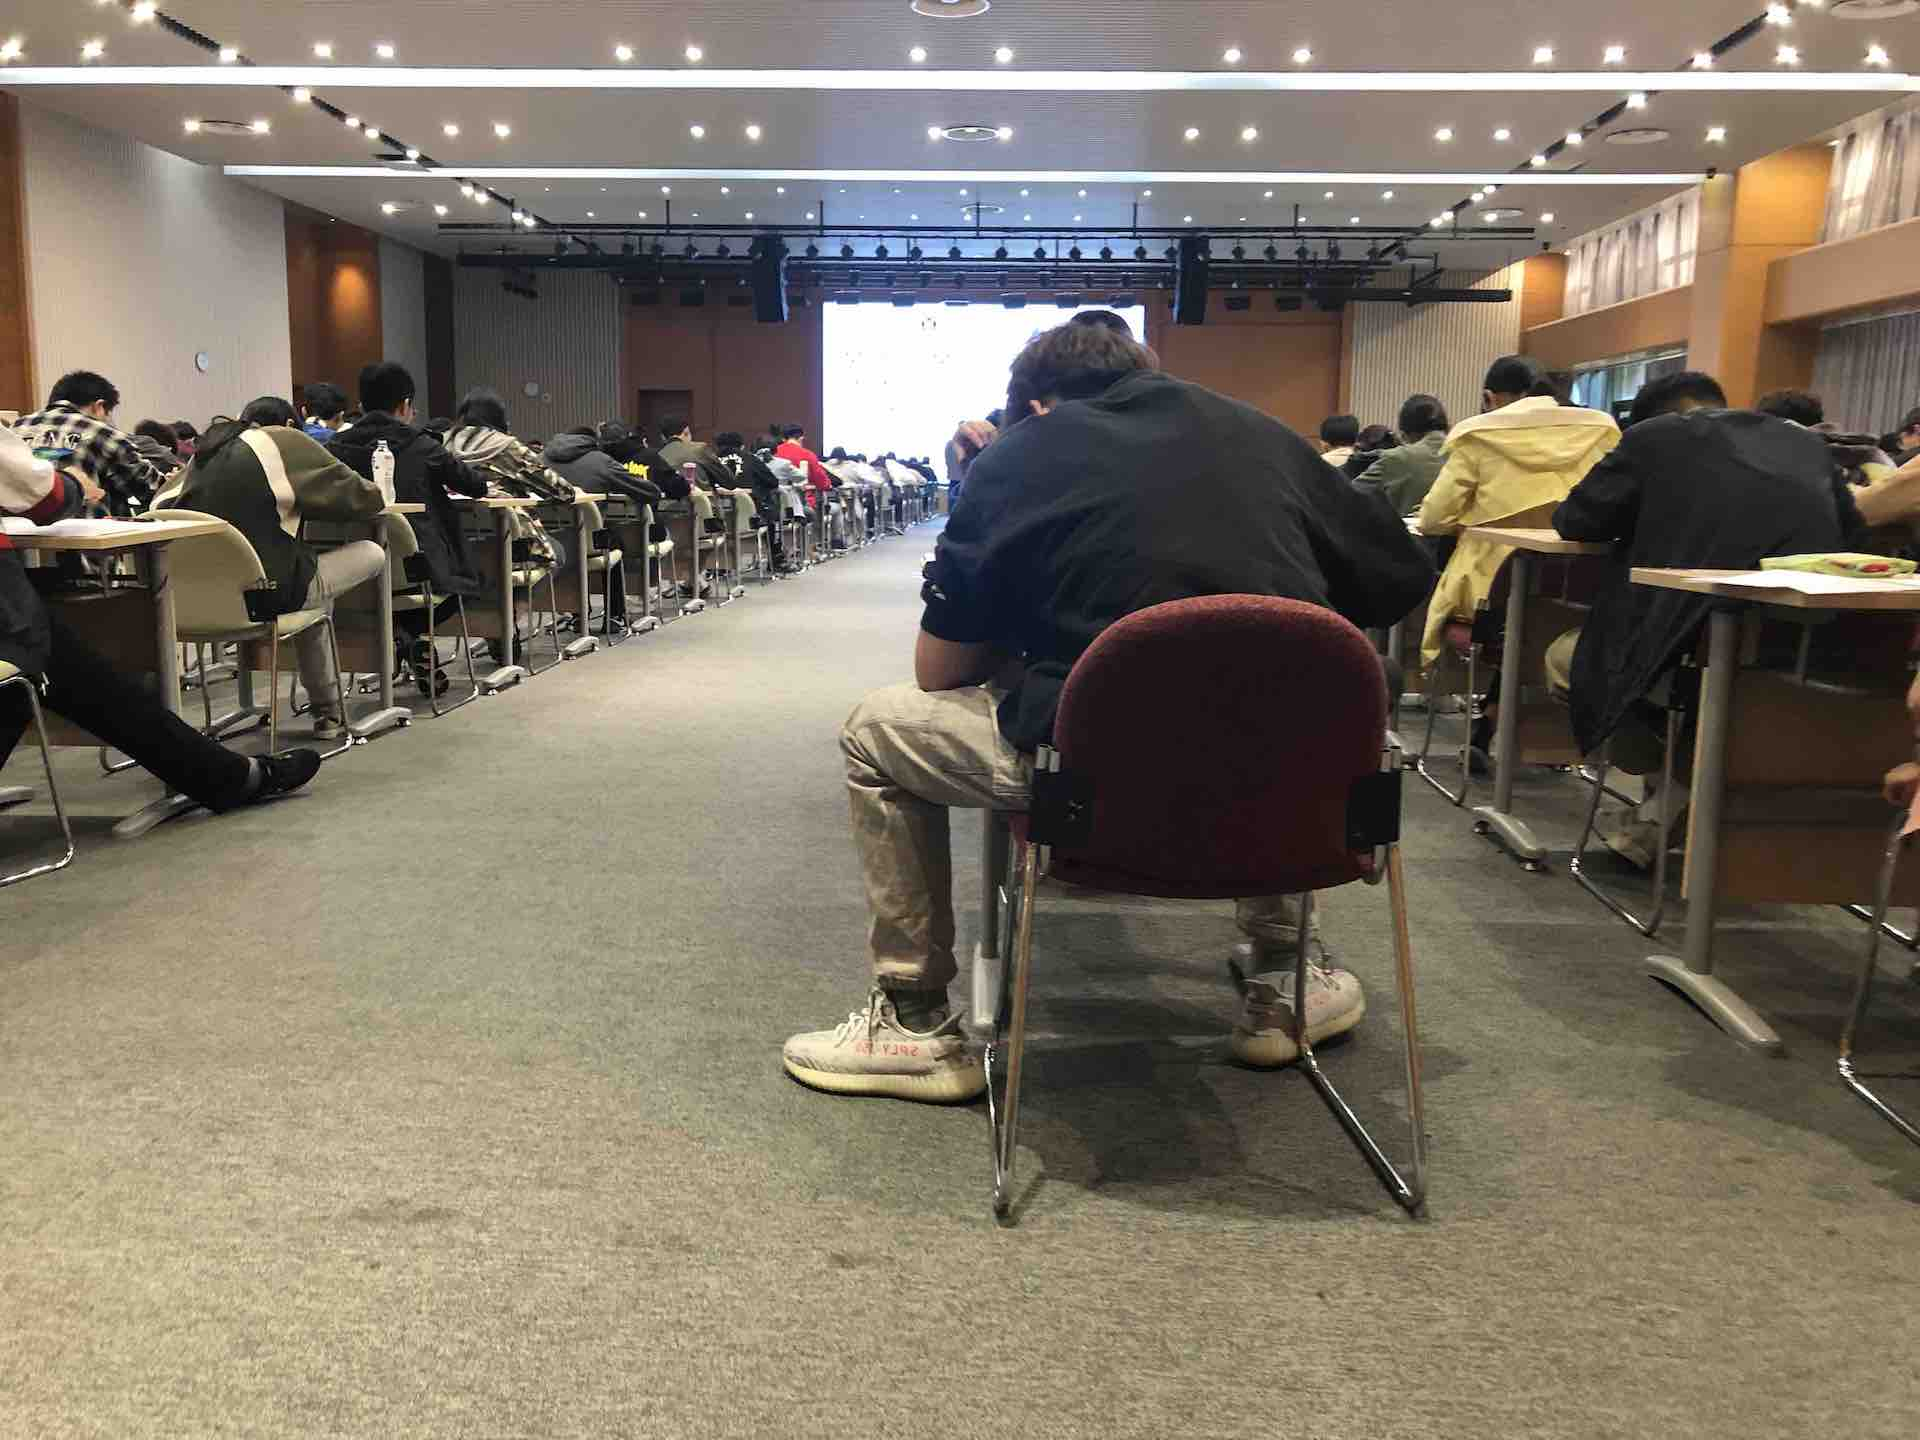
\includegraphics[width=0.9\columnwidth]{author-folder/Kai.Wu/invigilation.jpg}
    \caption{November 15, 2020, an exam hall on the G floor of the CB building, during invigilation}
\end{figure}

\begin{flushright}
    October 22, 2022 by \Wu \\
    Major update: December 30, 2022 by Yue Zhou \\
    GPT translation proofread by \Shiyao
\end{flushright}

% \begin{figure}[H]
%     \centering
%     \includegraphics[width=0.5\columnwidth]{author-folder/Kai.Wu/}
% \end{figure}

% \usepackage[export]{adjustbox}

% \item 
% \begin{minipage}{0.3\textwidth}
%     Text
% \end{minipage}
% \begin{minipage}{0.63\textwidth}
%     \begin{figure}[H]
%         \includegraphics[width=0.4\columnwidth, right]{author-folder/Kai.Wu/}
%     \end{figure}
% \end{minipage}

% \input{author-folder/Kai.Wu/.tex}
